\chapter{Introduction}\label{ch:introduction}
The Standard Model of particle physics, which describes the fundamental constituents of matter and their interactions, represents an unambiguous triumph of the scientific method. Its predictions have been verified to extraordinary precision. Its last missing piece, the Higgs boson, was discovered in 2012 \cite{Aad:2012tfa,Chatrchyan:2012xdj}, fifty years after it was predicted. This resulted in a Nobel prize for François Englert and Peter Higgs, and in much jubilation among the particle physics community. 

However, many questions still remain unanswered by the Standard Model. For example, it does not explain why neutrinos have masses, and does not contain a viable dark matter candidate. On a more abstract level, the square of the mass of the Higgs boson seems unnaturally finely tuned - this phenomenon is termed the \emph{hierarchy problem}, and we will revisit it in \autoref{sec:supersymmetry}. In fact, it is widely believed that the Standard Model is only a low-energy effective approximation to an underlying theory that is valid at higher energy scales.

To answer these questions, we must go beyond the Standard Model with new theories. These new theories often predict new fundamental particles and forces, which we can study using particle colliders, like the Large Hadron Collider (LHC), which lies on the border between Switzerland and France (\autoref{fig:LHC_schematic}).

\begin{figure}
  \centering
  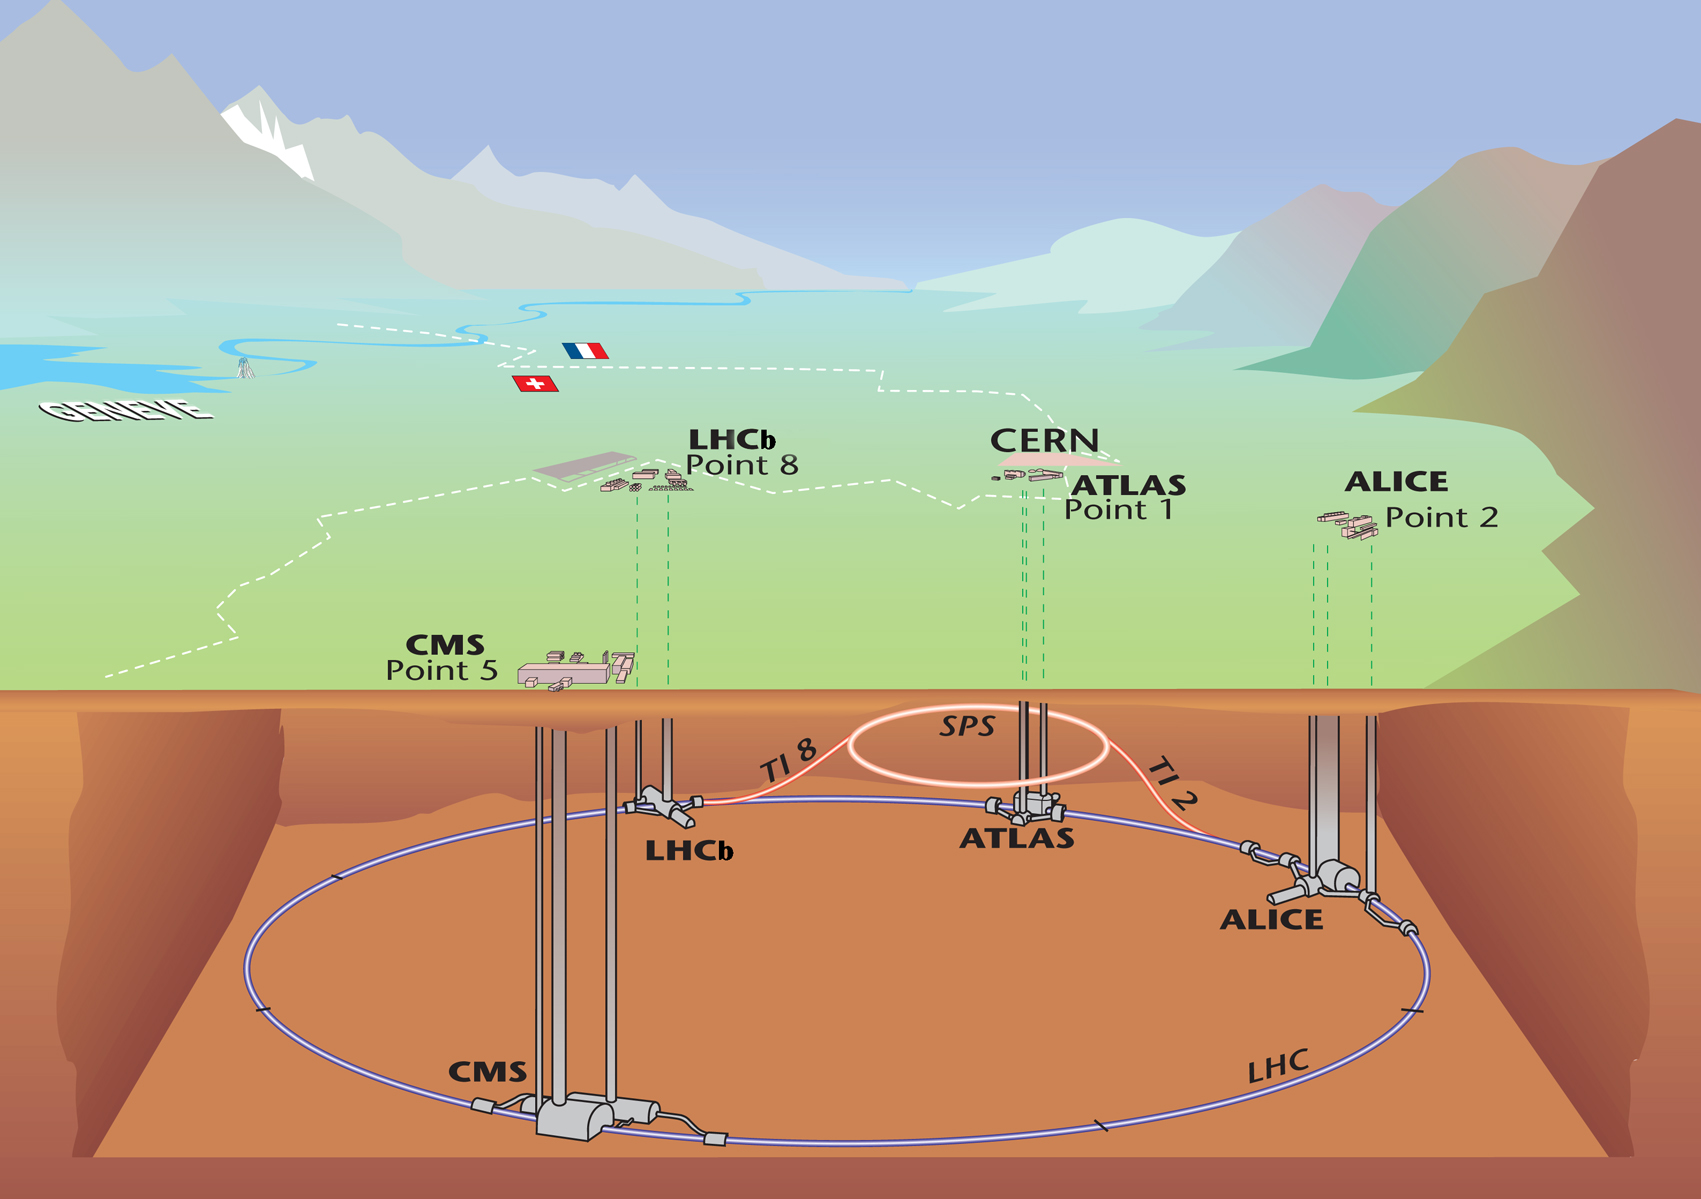
\includegraphics[width=0.9\textwidth]{images/LHC}
  \caption{Schematic diagram of the Large Hadron Collider, which lies on the border between Switzerland and France. \href{http://cds.cern.ch/journal/CERNBulletin/2008/38/News\%20Articles/1125888?ln=en}{(CERN)}}
  \label{fig:LHC_schematic}
\end{figure}

At these colliders, we collide particles at near-lightspeed, creating new particles that can be detected by extremely sophisticated detectors. One of the main challenges at particle colliders is that there are hundreds of millions of collisions every second, but only a small fraction of these will have signatures of new physics. In addition, there are a multitude of promising theories beyond the Standard Model, each possessing a large parameter space. However, performing a full experimental analysis for even a single point of this parameter space be very time consuming.

For this reason, existing theories must be constrained (or excluded entirely) by holding them up to the light of experimental evidence. Furthermore, we need to have a rough idea of what the most effective collider search strategies are before going ahead with a complete experimental analysis. This is where phenomenology steps in.

Phenomenology bridges the gap between theory and experiment - connecting the predictions of the former with the measurements of the latter. In this dissertation, we present three phenomenological analyses for finding physics beyond the Standard Model at current and future colliders. The structure of the dissertation is as follows.

\paragraph{Chapter \ref{ch:theory}} This chapter briefly reviews the theoretical background behind the collider analyses presented in this dissertation. We go over the particle content and gauge structure of the Standard Model, followed by a discussion of electroweak symmetry breaking. We briefly touch upon CKM mixing, asymptotic freedom, and quantum chromodynamics as well. This is followed by a discussion of the motivations, mass spectrum, and interactions of Two Higgs Doublet Models and the Minimal Supersymmetric Standard Model.

\paragraph{Chapter \ref{ch:ColliderPheno}} This chapter describes how to connect theoretical predictions and experimental observables. The design of a generic multipurpose detector for a hadron collider is discussed, followed by discussions of some of the kinematic variables that are relevant to our analyses. The concepts of hypothesis testing and statistical significance and briefly reviewed, and particle physics concerns are recast in the language of machine learning.

\paragraph{Chapter \ref{ch:LightChargedHiggs}} 
A new type of Higgs boson, known as the \emph{charged} Higgs boson $H^\pm$, arises naturally in the spectrum of $2$HDMs. Finding one of these would be an unmistakable sign of new physics beyond the Standard Model. The mass of this particle, $m_{H^\pm}$ is a free parameter in the theory. Searches for this particle can be divided into two broad categories - the first involving charged Higgs bosons lighter than the top quark, and the other dealing with charged Higgses heavier than the top quark. In this chapter, we examine the first scenario, with charged Higgses coming from the decay of top quarks that are either produced singly or in pairs. While experimental results from CMS and ATLAS  have placed a lower limit of 160 GeV for the mass of the charged Higgs boson in the context of the MSSM, these limits have been placed assuming that the charged Higgs decays solely via conventional channels to final states with SM particles. However, theories that predict charged Higgs typically predict other BSM particles as well. These can potentially be lighter than the charged Higgs, thus opening up new, `exotic' decay channels for it. For regions of parameter space with low values of the parameter $\tan\beta$, the rate of these exotic decays is much larger than the rate of the decays to SM particles, thus significantly weakening the limits set by the LHC. For a complete picture, we must take into account not only the conventional decay channels, but the exotic ones as well. In this chapter, we investigate the exotic decay of a charged Higgs to a lighter, neutral Higgs boson - either the pseudoscalar \emph{A} or the CP-even scalar \emph{H}, and a \emph{W} boson. 
We first perform a \emph{model-independent} analysis. That is, \emph{assuming} that $H^\pm$ decays exclusively to $AW^\pm/HW^\pm$, and that \emph{A/H} decays to a pair of tau leptons 8.6\% of the time, we set out to find the minimum rate of the signal process required for this analysis to discover it with a significance of 5$\sigma$, or exclude it with a significance of 1.96$\sigma$. This rate corresponds to the strength of the signal - the weaker the signal that can be probed by the analysis, the more powerful the analysis is. The model-independent limit on the signal strength can be translated into a limit on the branching ratio of the top quark to the charged Higgs, BR$(t\rightarrow H^\pm b$. We determined that the single top and the top pair channels could potentially set upper limits of 0.2\% and 0.3\% respectively on this branching ratio . For this analysis to discover the signal process, the branching ratio would have to be about three times higher than the aforementioned upper limits. These results can be translated into contours in the two-dimensional $m_{H^\pm}-\tan\beta$ plane in the parameter space of a Type-II $2$HDM that delineate regions that can be either discovered or excluded with this analysis. We also found that this analysis would be able to discover points with the charged Higgs mass $m_{H^\pm}$ between 155 and 165 GeV for $\tan\beta >$17, and the entire viable mass range for $\tan\beta <$6. We also found that almost the entire relevant region of the $m_{H^\pm}-\tan\beta$ plane can be excluded with this analysis, with the exception of the regions with very small mass differences between the charged Higgs and the top quark. In summary, we found that the exotic decay channel $H^\pm\rightarrow AW^\pm/HW^\pm$ probes a region of parameter space complementary to the region probed by standard decay channels (such as $H^\pm\rightarrow \tau\nu$), and is thus an important search channel to include in the search for charged Higgs bosons.
The results in this chapter have been published as an article in the Journal of High Energy Physics \citep{Kling2015c}, co-authored with Felix Kling and Shufang Su. While there has been some editing to achieve integration with the dissertation, there will inevitably be a substantial overlap between the chapter and the published article. The collider analysis for the top pair production channel, as well as the calculation of the limits was carried out by Felix, while analysis for the single top production channel was performed by the author of this dissertation.  

\paragraph{Chapter \ref{ch:ExoticHiggs}}
While the project that \autoref{ch:LightChargedHiggs} is based on dealt with the implications of additional, exotic decay channels opening up for charged Higgs bosons arising from extended scalar sectors at the LHC, the project that this chapter is based on is much more ambitious in scope, aiming for nothing less than a complete prospectus of exotic Higgs decay channels in $2$HDMs with large mass hierarchies. The authors of \citep{Kling2016} have presented a collection of promising $2$HDM benchmark planes for investigation at the LHC that take into account theoretical and experimental constraints, and highlight the complementarity between the different search channels. The end goal of this project is to perform detailed collider analyses to determine exclusion and discovery bounds for both the original benchmark planes at the 14 TeV LHC, as well as extended versions of them at a 100 TeV collider that, reflecting the higher obtainable mass reach. In this chapter, we present preliminary results based on collider analyses carried out for two of the benchmark planes, corresponding to the mass hierarchies $m_H < m_A = m_{H^\pm}$ and $m_A < m_H = m_{H^\pm}$. The exotic decay channels considered are $A\rightarrow HZ$ and $H^\pm\rightarrow HW^\pm$. The analyses in this chapter are based on boosted decision tree classifiers. Using this technique, we are able to exclude charged Higgses with masses up to 2 TeV, for neutral Higgses \emph{H} with masses up to 500 GeV, in the benchmark plane IIB suggested in \cite{Kling2016} through the decay mode $H^\pm\rightarrow AW^\pm$ at a 100 TeV collider. In addition, we are able to exclude neutral Higgses (\emph{A/H}) decaying via the channels $(A/H)\rightarrow (H/A)Z$ for parent masses up to about 3 TeV for a wide range of values of $\tan\beta$, keeping the daughter Higgs mass fixed at 200 GeV.

This work is being done in collaboration with Felix Kling, Huayang Song, Honglei Li, and Shufang Su. The results for the $A\rightarrow HZ$ channels have been obtained by Huayang and Honglei by using and extending analysis code originally written by Felix, while the results for the $H^\pm\rightarrow HW^\pm$ decay channel have been obtained by the author using code that builds upon that used for \autoref{ch:DM_100_TeV}. The Monte Carlo event samples for all the channels at 100 TeV were generated by the author on the University of Arizona computing cluster.

\paragraph{Chapter \ref{ch:DM_100_TeV}}
A 100 TeV proton-proton collider will be an extremely effective way to probe the electroweak sector of the Minimal Supersymmetric Standard Model (MSSM). In this chapter, we describe a search strategy for discovering pair-produced higgsino-like neutralinos $\tilde{\chi}_{2,3}^0$ that decay to the lightest neutralino $\tilde{\chi}_1^0$ (which we assume to be an almost pure bino). The lightest neutralino is a strong candidate for particle dark matter. We investigate the particular case in which the higgsinos decay via intermediate \emph{Z} and SM Higgs bosons \emph{h}, that in turn decay to a pair of leptons and a pair of \emph{b}-quarks respectively: 
$$\tilde{\chi}^0_{2,3}\tilde{\chi}^0_{3,2}\rightarrow (Z\tilde{\chi}^0)(h\tilde{\chi}_1^0)\rightarrow bbll+\tilde{\chi}_1^0\tilde{\chi}_1^0.$$
We performed two analyses simultaneously - the first using rectangular selection cuts on physically motivated kinematic observables known as razor variables, and the second using the same high-level observables, along with a few lower-level observables as input features for a Boosted Decision Tree Classifier. The results show that the machine learning technique performs substantially better than the regular rectangular selection cuts. With the machine learning analysis, we would be able to discover higgsinos up to a mass of 1.3 TeV, and exclude them to up to a mass of 1.8 TeV. Correspondingly, we can discover binos up to 900 GeV, and exclude them up to 1.3 TeV. The research for this chapter was carried out by the author under the guidance of Shufang Su, and forms the basis of a completed manuscript that will soon be submitted for publication in a peer-reviewed journal.

Finally, we conclude in \autoref{ch:Conclusion}, where we provide a summary of our findings and discuss prospects for future work.

%Generating these samples for hundreds of signal benchmark points and backgrounds with extremely large cross sections is not a trivial task (and even less so at 100 TeV), and requires careful management of computational resources. During the course of performing the research that comprises this dissertation, the author has developed a Python-based framework, \texttt{clusterpheno}, for event generation and analysis on a cluster. An advantage of using this over the CMS gridpack method is that the entire pipeline of MadGraph-Pythia-Delphes is integrated
